%

% Cal Poly Thesis
% 
% based on UC Thesis format
%
% modified by Mark Barry 2/07.
%




\documentclass[12pt]{ucthesis}



\newif\ifpdf
\ifx\pdfoutput\undefined
    \pdffalse % we are not running PDFLaTeX
\else
\pdfoutput=1 % we are running PDFLaTeX
\pdftrue \fi

\usepackage{url}
\ifpdf

    \usepackage[pdftex]{graphicx}
    % Update title and author below...
    \usepackage[pdftex,plainpages=false,breaklinks=true,colorlinks=true,urlcolor=blue,citecolor=blue,%
                                       linkcolor=blue,bookmarks=true,bookmarksopen=true,%
                                       bookmarksopenlevel=3,pdfstartview=FitV,
                                       pdfauthor={!!Author goes here!!},
                                       pdftitle={!!Title goes here!!},
                                       pdfkeywords={thesis, masters, cal poly}
                                       ]{hyperref}
    %Options with pdfstartview are FitV, FitB and FitH
    \pdfcompresslevel=1

\else
    \usepackage{graphicx}
\fi

\graphicspath{ {Images/} }

\usepackage{amssymb}
\usepackage{amsmath}
\usepackage[letterpaper]{geometry}
\usepackage[overload]{textcase}

%\usepackage[disable]{todonotes} % notes not showed
\usepackage[draft]{todonotes}   % notes showed



\bibliographystyle{abbrv}

\setlength{\parindent}{0.25in} \setlength{\parskip}{6pt}

\geometry{verbose,nohead,tmargin=1.25in,bmargin=1in,lmargin=1.5in,rmargin=1.3in}

\setcounter{tocdepth}{2}


% Different font in captions (single-spaced, bold) ------------
\newcommand{\captionfonts}{\small\bf\ssp}

\makeatletter  % Allow the use of @ in command names
\long\def\@makecaption#1#2{%
  \vskip\abovecaptionskip
  \sbox\@tempboxa{{\captionfonts #1: #2}}%
  \ifdim \wd\@tempboxa >\hsize
    {\captionfonts #1: #2\par}
  \else
    \hbox to\hsize{\hfil\box\@tempboxa\hfil}%
  \fi
  \vskip\belowcaptionskip}
\makeatother   % Cancel the effect of \makeatletter
% ---------------------------------------




\begin{document}

% Declarations for Front Matter

% Update fields below!
\title{This is the Title of My Thesis2}
\author{Jason Banich}
\degreemonth{March} \degreeyear{2016} \degree{Master of Science}
\defensemonth{March} \defenseyear{2016}
\numberofmembers{3} \chair{Dr. John Seng, Professor of Computer Science} \othermemberA{Dr. Franz Kurfess} \othermemberB{Person3, Ph.D.} \field{Computer Science} \campus{San Luis Obispo}
\copyrightyears{seven}


\todo[inline]{COMMMENTS ARE ENABLED OH NOOOOOOOO}

\maketitle

\begin{frontmatter}

% Custom made for Cal Poly (by Mark Barry, modified by Andrew Tsui).
\copyrightpage

% Custom made for Cal Poly (by Andrew Tsui).
\committeemembershippage

\begin{abstract}
\todo[inline]{This is a to do note}
It can be difficult to guide yourself across a crosswalk successfully when your visual capabilities are limited. This can be an everyday issue for someone with impaired vision. This paper aims to help alleviate that issue by focusing on zebra stripe crosswalks and coming up with an algorithm that can quickly and accurately identify and help guide a user across the crosswalk using a handheld device such as a phone. The image is identified as being part of a crosswalk or not, and then the user could be given feedback directing them back towards the crosswalk if they are off-course.

\todo[inline]{Add more/redo}

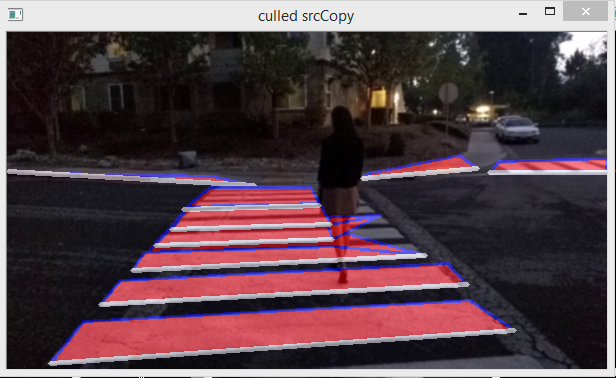
\includegraphics[width=10cm, angle=45]{testimg}

\end{abstract}

\begin{acknowledgements}
I would like to acknowledge my parents for supporting me through college.
\todo[inline]{WRITE AN ACTUAL THING MAYBE}
\end{acknowledgements}


\tableofcontents


\listoftables

\listoffigures

\end{frontmatter}

\pagestyle{plain}




\renewcommand{\baselinestretch}{1.66}


% ------------- Main chapters here --------------------





\chapter{Introduction}
\label{intro}


This is the introduction.

\chapter{Background}
\section{Types of crosswalks}

\begin{figure}
\begin{center}
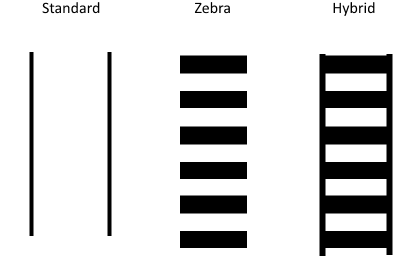
\includegraphics[width=10cm]{TypesOfXwalks.png}
\captionfonts
\caption[This is a figure]{A few types of crosswalks}
\label{fig:TypesOfXwalksFig}
\end{center}
\end{figure}

\begin{figure}
\begin{center}
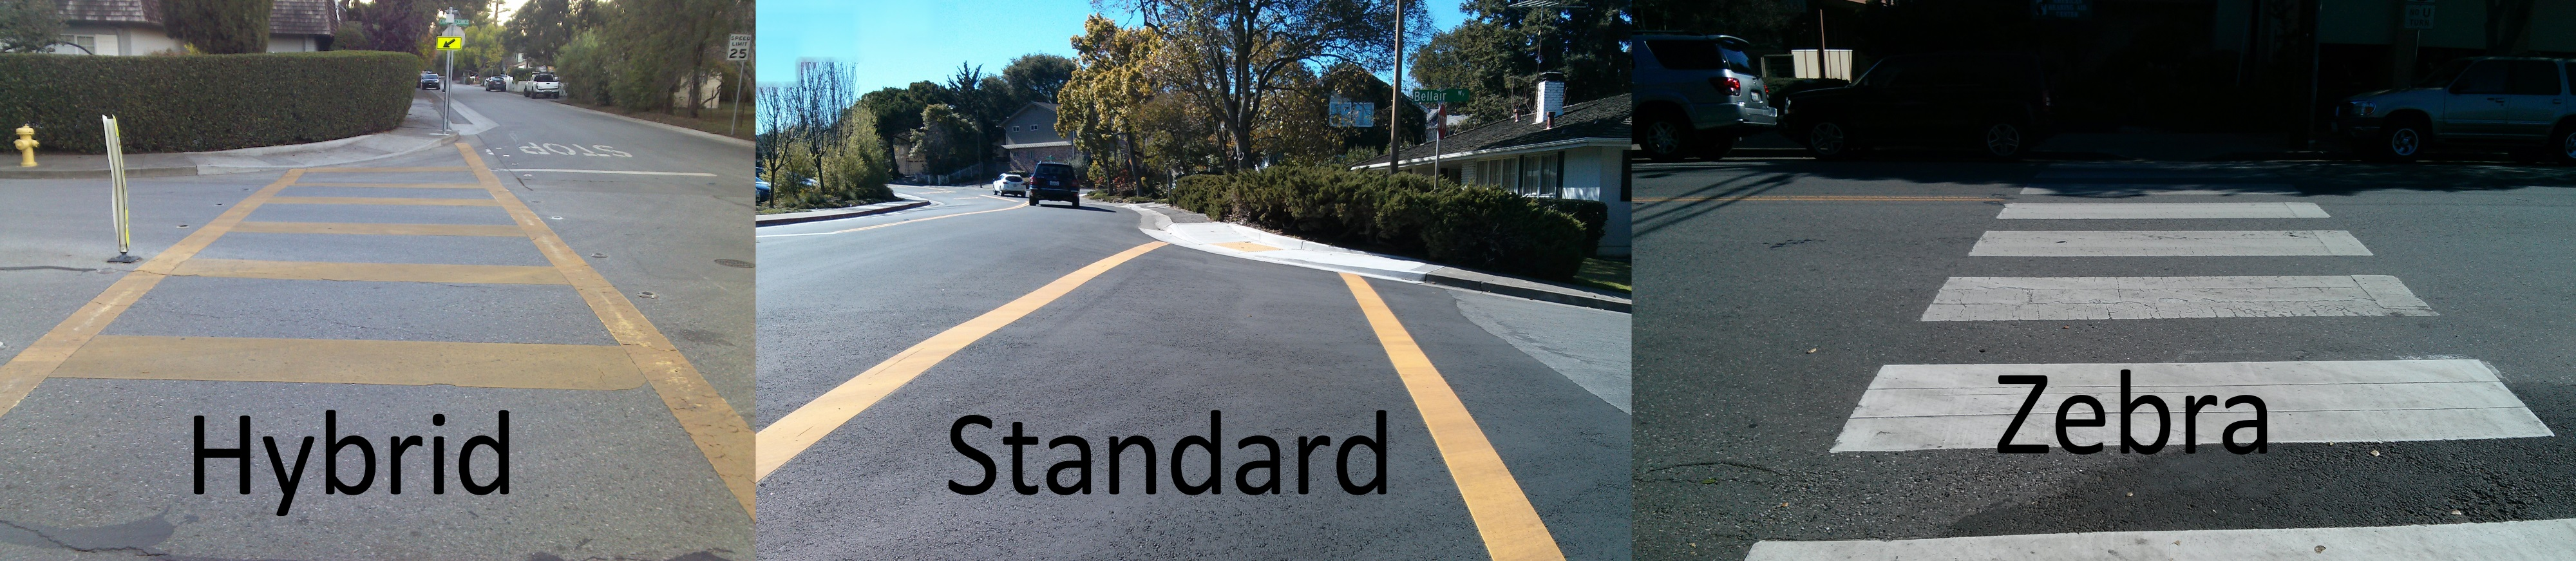
\includegraphics[width=13cm]{All3Types.jpg}
\captionfonts
\caption[This is a figure]{Real world samples of the types of crosswalks}
\label{fig:TypesOfXwalksRealFig}
\end{center}
\end{figure}

\begin{figure}
\begin{center}
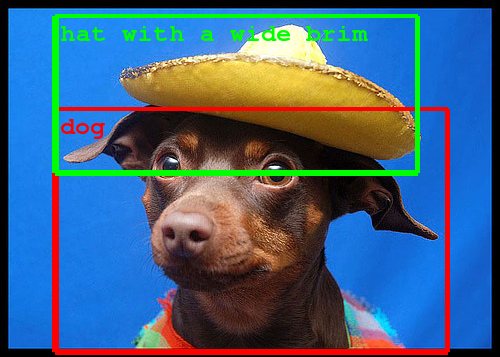
\includegraphics[width=10cm]{DogWithHat.PNG}
\captionfonts
\caption[This is a figure]{Neural network classification result\cite{christianszegedy2014}}
\label{fig:DogWithHat}
\end{center}
\end{figure}

There are many types of crosswalks (See figure \ref{fig:TypesOfXwalksFig} and \ref{fig:TypesOfXwalksRealFig} for some examples), with the main two being zebra stripe crosswalks and standard two line crosswalks. Two line crosswalks are more commonly used due to their simplicity, but zebra crosswalks are often used in more critical intersections due to their benefits in visibility \cite{crosswalkTypeEvaluation}. Using vision processing to recognize the boundaries of two line crosswalks has essentially been done many times over, because there is no real difference between processing a two line crosswalk and processing the driving lane of a car.
\section{Neural Networks}
Neural network are a type of machine learning that has been used recently for many vision applications such as image classification (See figure \ref{fig:DogWithHat}) and LIST ANOTHER \cite{christianszegedy2014}. Neural Networks are well suited for many data sets that include lots of information that could be very difficult to manually train a computer to categorize. They can even be used to help determine what signals from the brain to use to trigger prosthetic limbs to move by measuring results of brain probes in rats \cite{ratNeural}.

\todo[inline]{Minor summary of neural networks}



\chapter{Previous Work}
\label{previous-work}

LaTeX is a document markup language and document preparation system for the TeX typesetting program.


\chapter{Algorithm}
\section{Overview}
\label{Overview}

\begin{figure}
\begin{center}
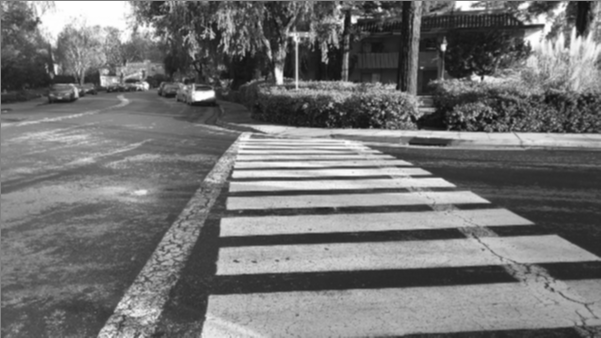
\includegraphics[width=7cm]{SlightlyBlurredInput.png}
\captionfonts
\caption[This is a figure]{Input image blurred and converted to grayscale}
\label{fig:SlightlyBlurred}
\end{center}
\end{figure}

\begin{figure}
\begin{center}
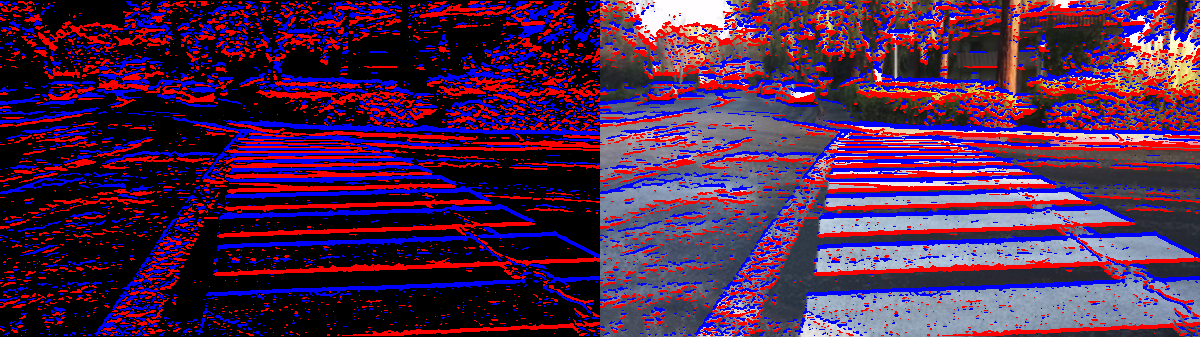
\includegraphics[width=14cm]{TopAndBottomSobel.png}
\captionfonts
\caption[This is a figure]{Sobel derivative of the image - positive values colored red, negative values colored blue}
\label{fig:TopAndBottomSobel}
\end{center}
\end{figure}

\begin{figure}
\begin{center}
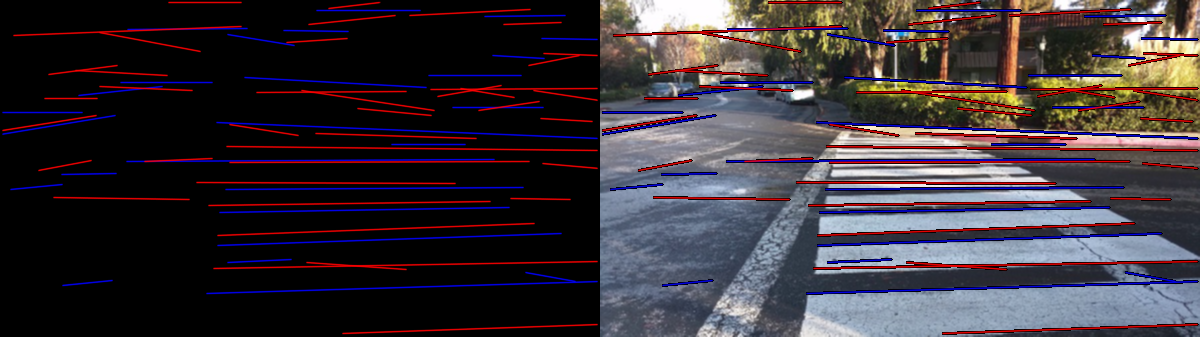
\includegraphics[width=14cm]{HoughLinesAfterMerge.png}
\captionfonts
\caption[This is a figure]{Lines detected using Hough transform on image from figure \ref{fig:TopAndBottomSobel} - blue is potential crosswalk top lines, red is potential crosswalk bottom lines}
\label{fig:HoughLinesAfterMerge}
\end{center}
\end{figure}

\begin{figure}
\begin{center}
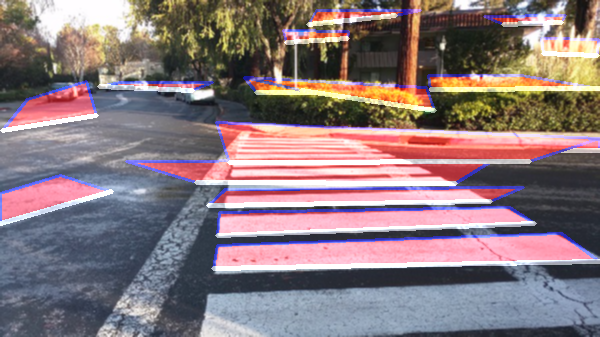
\includegraphics[width=7cm]{UnculledStriplets.png}
\captionfonts
\caption[This is a figure]{All of the striplets detected after running the constraints on all the input lines from figure \ref{fig:HoughLinesAfterMerge}}
\label{fig:UnculledStriplets}
\end{center}
\end{figure}

Description of Algorithm for striplet detection:

Following the Figure ground paper, the frame is blurred slightly, and then converted to grayscale (See figure \ref{fig:SlightlyBlurred}). The Sobel derivative is taken in the Y direction, giving us just the changes in the Y direction (PICTURE). These points are either negative or positive, which represents whether they are going from dark to light, or light to dark, giving us pixels that can be either the bottom of the top of the crosswalk. These are potential edges of crosswalks in the image (See figure \ref{fig:TopAndBottomSobel}). Hough line transform is then used to detect lines (figure \ref{fig:HoughLinesAfterMerge}). The generated lines are either defined as potential crosswalk top edges, or bottom edges. These potential edges are matched up against other edges (top vs bottom edges) to determine if they fit certain criteria to be considered as a striplet. A striplet is defined as an area bounded by a top and bottom line that follows certain constraints. The constraints used in the paper this technique is based on \cite{jamesm.coughlanhuiyingshen2006} are the same as used here: Top line is above bottom line in the image, the two lines' slopes are very similar, the vertical width of the generated striplet is the between a defined cutoff values, and the two lines have sufficient X overlap. If all of these are true, then it is returned as a striplet (See figure \ref{fig:UnculledStriplets}). 

I'm going to say what is currently being done here, and specify the potential future options. 

The three striplets with the highest intensities are then selected and compared. If two of the chosen striplets satisfy these constraints, then the image is declared to have a zebra crosswalk inside of it: The average slope of the two striplets match, the horizontal pixel overlap is within acceptable ranges, the lower striplet is wider, and the Y ranges can't overlap (or the overlap is extremely mineral). If all of these pass for two of the striplets, then the image is declared to be a crosswalk. If all of the constraints fail to pass, then the image is not a crosswalk. 


\section{Neural}

Once the striplets are detected, they were all marked as being part of a crosswalk or not. Then assorted types of data about them was computed and saved for the neural network training. Examples of metrics used were lengths of top and bottom of the crosswalk, the difference in length between them, the variance and standard deviation of the pixel intensity, etc. The neural network was then trained with many iterations over the training data. There was a very low chance of a false positive, so 

\section{Identifying crosswalk edges}
Once the neural network was trained, then each striplet in the image was determined to be likely part of the crosswalk or not. The striplets determined to likely be part of the crosswalk then had their left and right points run through a RANSAC detection algorithm to pick the best fit line for each side. 
\todo[inline]{CODE NOT YET DONE}
Those lines were then blended across multiple frames in order to attempt a more accurate edge of the crosswalk. 

\chapter{Results}
\label{results}

\todo[inline]{Need a bunch of data here, easy to get}

\todo[inline]{GRAB THE FINAL Numbers}
I had  10 input videos and 1000 input frames, which resulted in 8000 striplets for training. I kept separate videos that were only to be used for testing, never for training. There were 10 test videos, totalling in 300 input frames and 2400 detected striplets. After training the neural network, and running the neural network prediction on the output videos, 71\% of the crosswalks striplets were correctly identified as striplets, with a 92\% rate of a positive identification of a crosswalk striplet being correct. 
\todo[inline]{grab final percentages}


\chapter{Future Work}
\label{future work}

\section{Conversion to phone app}

The project was written entirely in the C++ libraries provided by OpenCV, which luckily can be ported almost directly to a mobile app without too many changes. There are many areas of improvement that could be implemented once access is given to the phone sensors. The current algorithm assumed that the photos were taken parallel to the horizon, but with access to a phone's sensors, the image frames could be adjusted such that they are guaranteed to be in the correct orientation. The accelerometer and gyroscope sensors could also be used to help track movement as the user crosses a crosswalk, confirming what the algorithm is telling us and assisting in the user's trajectory. Other mobile technologies such as Project Tango by Google \cite{projectTango} could be used as well to help with spacial awareness and other factors such as detecting objects in the way that need to be avoided. Once the program is converted to a mobile app, there are many interesting ways that it could progress.

\section{Crosswalks with shadows}

As this project did not cover crosswalks with shadows, future work could be done to adapt the project so it can work properly with crosswalks that have shadows inside of them. The current algorithm would hit a couple of snags with shadows, one being the Hough line transform might have issues because shadows naturally are strong lines, and another being that some of the neural network training parameters might be drastically different with shadows inside of the striplets. 

One way to go about that might be shadow removal algorithms that would remove the shadows so that the main algorithm doesn't have to account for them at all, which would possibly be the simplest solution in terms of code, but potentially not the fastest. It has been done many times before though, so there would be a lot of different ways to try \cite{shadowRemoval}. Another solution may be to try modifying the current algorithm to account for the shadows, which would involve likely modifying the Hough lines grouping, as well as using different or modified training parameters in addition to another set of training data including crosswalks with different types of shadows at different times of day. 

\section{Performance Improvements}

The algorithm definitely contains some areas where the performance could be improved. In this proof of concept, the speed isn't as important, so the algorithm is not as optimized as it could be. If it is ported to a phone app, the optimizations would become necessary for a real world optimization.
\subsection{Multithreading}
One specific improvement would be to take advantage of multiple cores in order to process multiple frames at the same time, which would improve the throughput and allow greater accuracy due to averaging the results of frames that are immediately next to each other, as well as being able to average more frames together. 
The current implementation running on a decent PC can run at around 1.6 frames per second, and would scale almost linearly with the number of cores, so if one core is 1.6 frames per second, then two would be 3.2 frames per second, so it is a very 
\todo[inline]{Finish mutlithreading}

\subsection{another one}




% ------------- End main chapters ----------------------

\clearpage
\bibliography{bibliography}
\bibliographystyle{plain}
%\addcontentsline{toc}{chapter}{Bibliography}

\end{document}
